\documentclass{article}

\usepackage[utf8]{inputenc}

\usepackage[russian]{babel}

\usepackage{graphicx}
\graphicspath{{pictures/}}
\DeclareGraphicsExtensions{.pdf,.png,.jpg}
\usepackage[unicode, pdftex]{hyperref}

\begin{document}

\begin{titlepage}
  \thispagestyle{empty}
  \centerline {Санкт-Петербургский политехнический университет}
  \centerline { им. Петра Великого}
  \centerline { }
  \centerline {Институт прикладной математики и механики} 
  \centerline {Кафедра "Прикладная математика"}
  \vfill
  \centerline{\textbf{Отчёт}}
  \centerline{\textbf{по лабораторной работе №1}}
  \centerline{\textbf{по дисциплине}}
  \centerline{\textbf{"Математическая статистика"}}
  \vfill
  \hfill
  \begin{minipage}{0.45\textwidth}
  Выполнил студент:\\
  Дроздова Дарья Александровна\\
  группа: 3630102/80401 \\
  \\
  Проверил:\\
  к.ф.-м.н., доцент \\
  Баженов Александр Николаевич
  \end{minipage}
  \vfill
  \centerline {Санкт-Петербург}   
  \centerline {2021 г.}  
\end{titlepage}

\newpage
\setcounter{page}{2}
\tableofcontents

\newpage
\listoffigures

\newpage
\section{Постановка задачи}
  Для 5 распределений:
  \begin{itemize}
    \item Нормальное распределение: $N(x,0,1)$
    \item Распределение Коши: $C(x,0,1)$
    \item Распределенеие Лапласа: $L(x,0,\sqrt{2})$
    \item Распределение Пуассона: $P(k,10)$
    \item Равномерное распределение: $U(x,-\sqrt{3}, \sqrt{3})$
  \end{itemize}
  Сгенерировать выборки мощностью 10, 50 и 1000 элементов. Построить на одном рисунке гистограмму и график плотности распределения
  
\newpage
\section{Теория}

\subsection{Нормальное распределение}
Нормальным называется распределение вероятностей, которое для одномерного случая задаётся функцией Гаусса. Нормальное распределение обозначается: ($N(x, \mu, \sigma^2)$), где $\mu$ - математическое ожидание, $\sigma^2$ - дисперсия. Плотность вероятностей нормального распределения определяется по формуле:
\begin{equation}
f(x)=\frac{1}{\sigma \sqrt{2\pi}}\exp(-\frac{(x-\mu)^2}{2\sigma^2})
\label{eq:1}
\end{equation}
В нашем случае $N(x,0,1)$, значит математическое ожидание $\mu=0$, дисперсия $\sigma^2=1$. Следовательно формула (\ref{eq:1}) плотности вероятности примет вид: 
\begin{equation}
f(x)=\frac{1}{\sqrt{2\pi}}e^{-\frac{x^2}{2}}
\label{eq:2}
\end{equation}

\subsection{Распределение Коши}
Распределение Коши обозначается, как $C(x, x_0, \gamma)$, где $x_0$ - параметр сдвига, $\gamma$ - параметр масштаба. Распределение Коши не имеет математического ожидания и дисперсии. Плотность данного распределения определяется по формуле:
\begin{equation}
f(x)=\frac{1}{\pi}[\frac{\gamma}{(x-x_0)^2+\gamma^2}]
\label{eq:3}
\end{equation}
По условию $C(x,0,1)$, значит $x_0=0, \gamma=1$, тогда формула плотности вероятности (\ref{eq:3}) будет иметь вид
\begin{equation}
f(x)=\frac{1}{\pi}\frac{1}{x^2+1}
\label{eq:4}
\end{equation}

\subsection{Распределение Лапласа}
Распределение Лапласа - непрерывное распределение случайной величины, обозначается как $L(x,\beta, \alpha)$, где $\alpha$ - коэффициент масштаба, $\beta$ - коэффициент сдвига. Математическое ожидание $\mu$ равняется $\mu=\beta$, а дисперсия - $\sigma^2=\frac{2}{\alpha^2}$. Плотность вероятности данного распределения определяется по формуле
\begin{equation}
f(x)=\frac{\alpha}{2}e^{-\alpha|x-\beta|}
\label{eq:5}
\end{equation}
В нашем случае $L(x,0,\sqrt{2})$, значит $\beta=0, \alpha=\sqrt{2}$, значит функция плотности вероятности (\ref{eq:5}) примет вид
\begin{equation}
f(x)=\frac{1}{\sqrt{2}}e^{-\sqrt{2}|x|}
\label{eq:6}
\end{equation}

\subsection{Распределение Пуассона}
Дискретная случайная величина имеет распределение Пуассона $P(k,\lambda)$ с параметром $\lambda$, если плотность вероятности определяется по формуле
\begin{equation}
f(x)=\frac{\lambda^k}{k!}e^{-\lambda}
\label{eq:7}
\end{equation}
По условию $P(k,10)$, т. е. $\lambda=10$, следовательно плотность вероятности (\ref{eq:7}) будет определяться по формуле
\begin{equation}
f(x)=\frac{10^k}{k!}e^{-10}
\label{eq:8}
\end{equation}

\subsection{Равномерное распределение}
Рассмотрим некоторый конечный промежуток $[a,b]$. Говорят, что величина распределена равномерно, если плотность распределения постоянна внутри данного отрезка и нулевая вне него. При этом функция плотности вероятности определяется как
\begin{equation}
f(x)=\left \{\ \begin{array}{rcl}
\frac{1}{b-a}, & x\in[a,b] \\
0, & x \notin [a,b] \\
\end{array}\right.
\label{eq:9}
\end{equation}
По условию рассматриваем отрезок $[-\sqrt{3},\sqrt{3}]$, значит плотность вероятности (\ref{eq:9}) определяется как

\begin{equation}
f(x)=\left \{\ \begin{array}{rcl}
\frac{1}{2\sqrt{3}}, & x\in[-\sqrt{3},\sqrt{3}] \\
0, & x \notin [-\sqrt{3},\sqrt{3}] \\
\end{array}\right.
\label{eq:10}
\end{equation}

\newpage
\section{Реализация}
Лабораторная работа выполнена на языке программирования Python в среде разработки PyCharm с использованием библиотек: numpy, skipy для построения выборок и вычислния плотностей вероятности, для построения графиков и гистограмм использовалась библиотека pyplot.
\\
Код программы расположен в репозитории GitHub по ссылке: \url{https://github.com/Drozdova-Daria/Math_Stat_Lab1}
\newpage
\section{Результаты}

\subsection{Нормальное распределение}
\begin{figure}[h]
\center{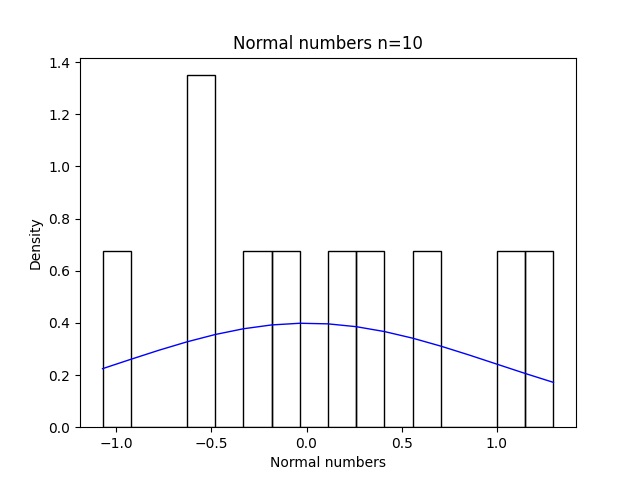
\includegraphics[scale=0.28]{Normal10}}
\caption{Нормальное распределение (\ref{eq:2}) для выборки мощности 10}
\end{figure}
\begin{figure}[h]
\center{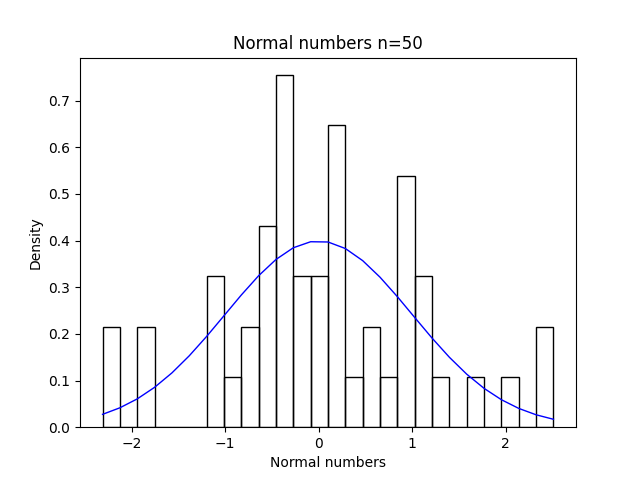
\includegraphics[scale=0.28]{Normal50}}
\caption{Нормальное распределение (\ref{eq:2}) для выборки мощности 50}
\end{figure}
\begin{figure}[h]
\center{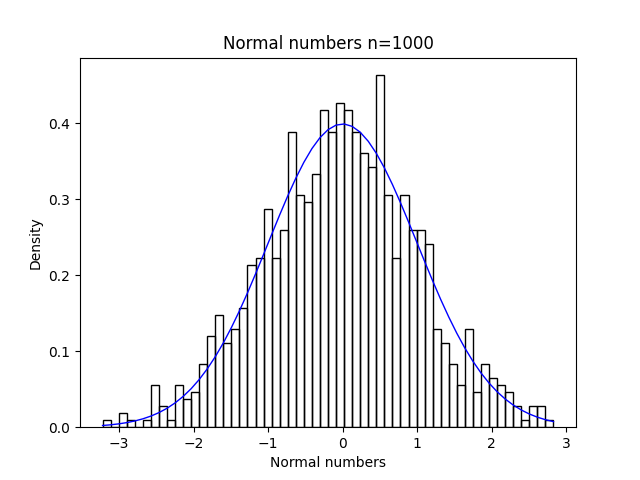
\includegraphics[scale=0.28]{Normal1000}}
\caption{Нормальное распределение (\ref{eq:2}) для выборки мощности 1000}
\end{figure}

\newpage
\subsection{Распределение Коши}
\begin{figure}[h]
\center{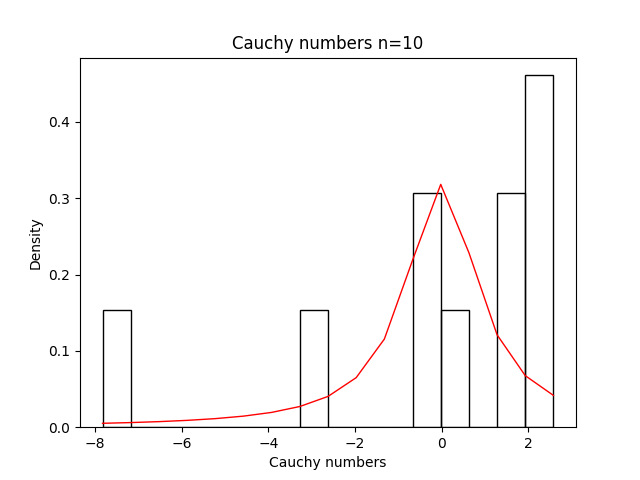
\includegraphics[scale=0.28]{Cauchy10}}
\caption{Распределение Коши (\ref{eq:4}) для выборки мощности 10}
\end{figure}
\begin{figure}[h]
\center{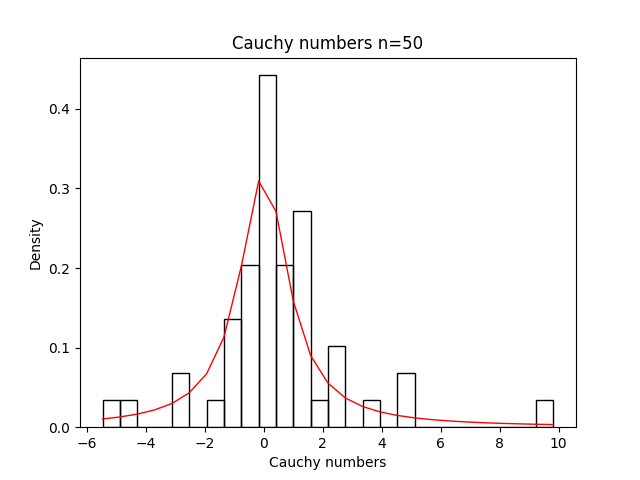
\includegraphics[scale=0.28]{Cauchy50}}
\caption{Распределение Коши (\ref{eq:4}) для выборки мощности 50}
\end{figure}
\begin{figure}[h]
\center{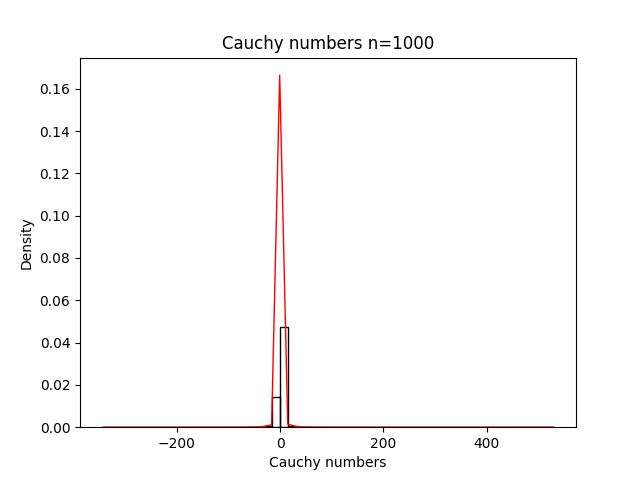
\includegraphics[scale=0.28]{Cauchy1000}}
\caption{Распределение Коши (\ref{eq:4}) для выборки мощности 1000}
\end{figure}

\newpage
\subsection{Распределенеие Лапласа}
\begin{figure}[h]
\center{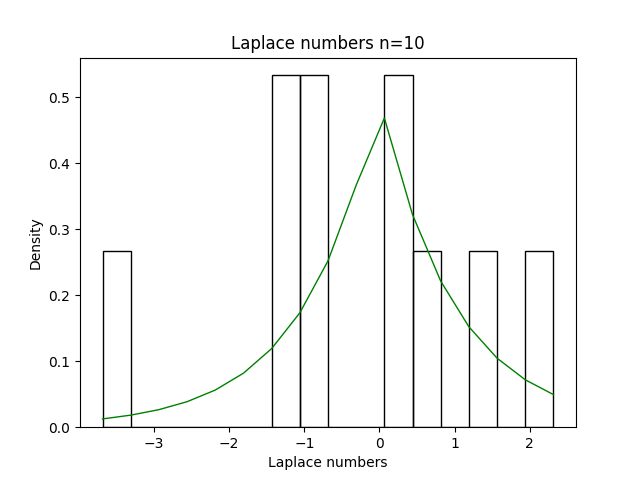
\includegraphics[scale=0.28]{Laplace10}}
\caption{Распределенеие Лапласа (\ref{eq:6}) для выборки мощности 10}
\end{figure}
\begin{figure}[h]
\center{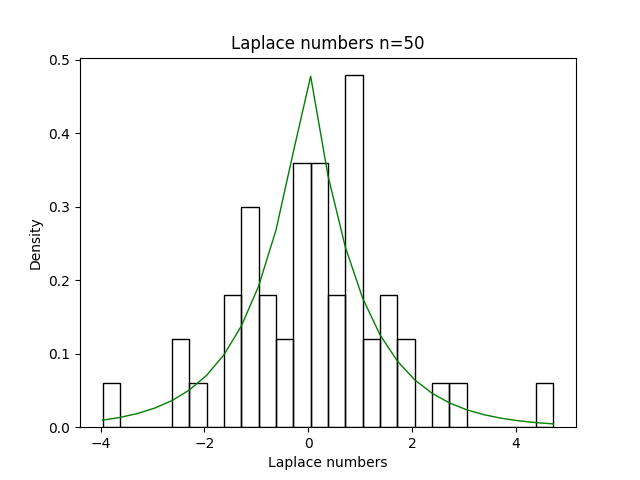
\includegraphics[scale=0.28]{Laplace50}}
\caption{Распределенеие Лапласа (\ref{eq:6}) для выборки мощности 50}
\end{figure}
\begin{figure}[h]
\center{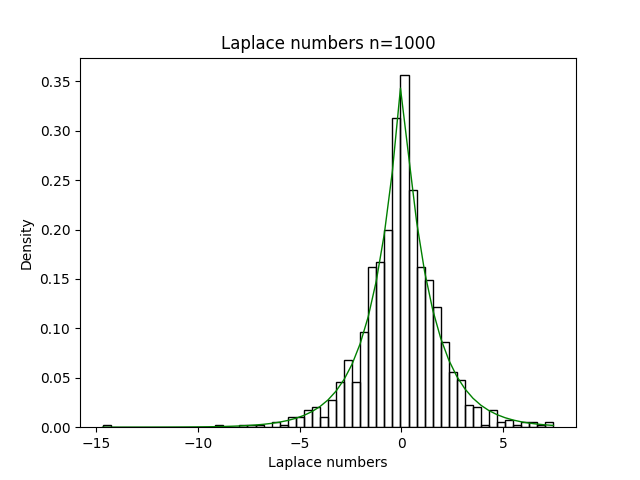
\includegraphics[scale=0.28]{Laplace1000}}
\caption{Распределенеие Лапласа (\ref{eq:6}) для выборки мощности 1000}
\end{figure}

\newpage
\subsection{Распределение Пуассона}
\begin{figure}[h]
\center{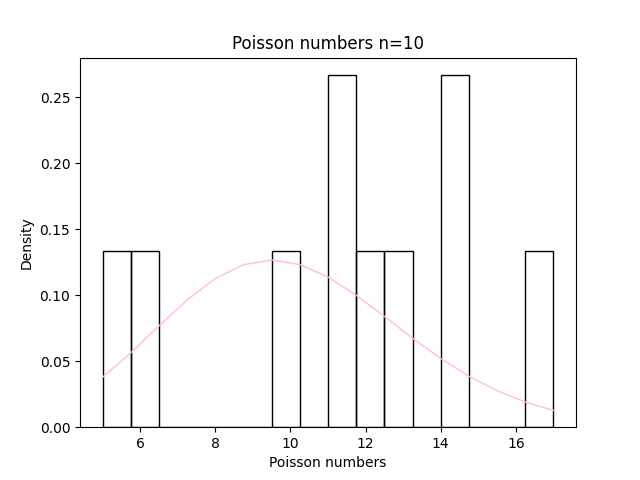
\includegraphics[scale=0.28]{Poisson10}}
\caption{Распределение Пуассона (\ref{eq:8}) для выборки мощности 10}
\end{figure}
\begin{figure}[h]
\center{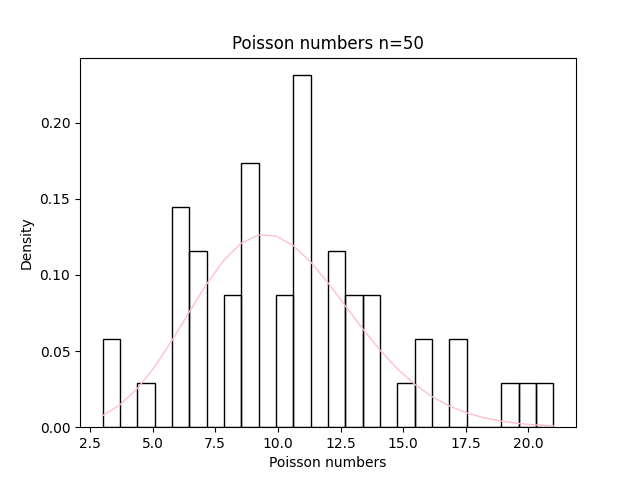
\includegraphics[scale=0.28]{Poisson50}}
\caption{Распределение Пуассона (\ref{eq:8}) для выборки мощности 50}
\end{figure}
\begin{figure}[h]
\center{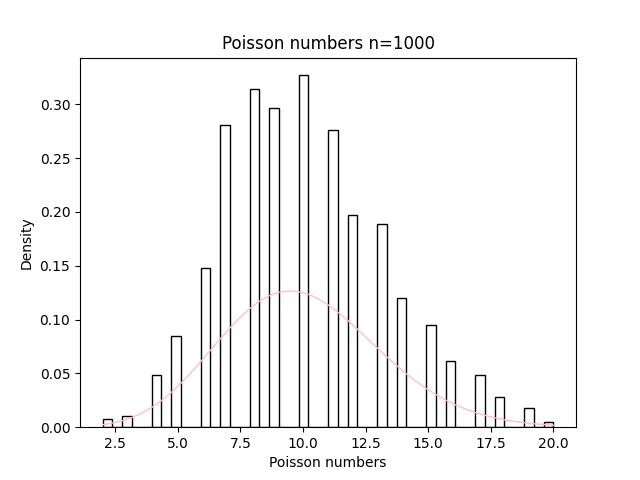
\includegraphics[scale=0.28]{Poisson1000}}
\caption{Распределение Пуассона (\ref{eq:8}) для выборки мощности 1000}
\end{figure}

\newpage
\subsection{Равномерное распределение}
\begin{figure}[h]
\center{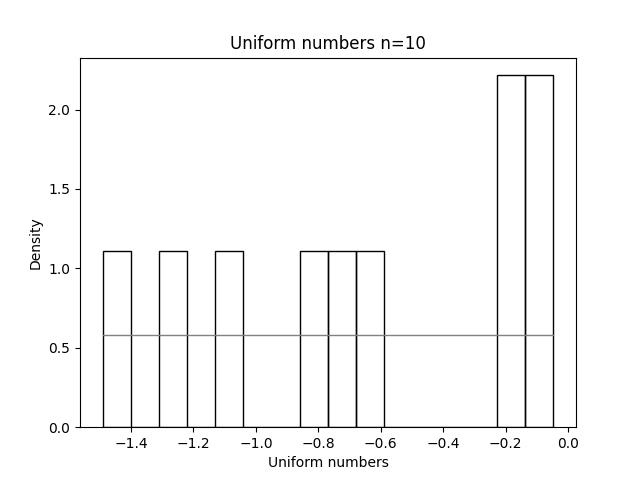
\includegraphics[scale=0.28]{Uniform10}}
\caption{Равномерное распределение (\ref{eq:10}) для выборки мощности 10}
\end{figure}
\begin{figure}[h]
\center{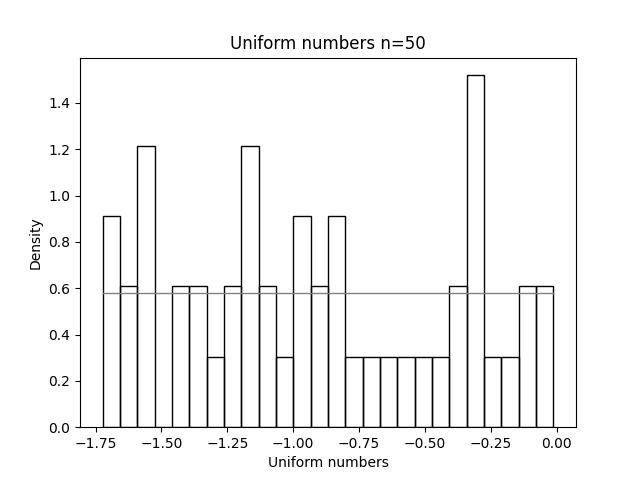
\includegraphics[scale=0.28]{Uniform50}}
\caption{Равномерное распределение (\ref{eq:10}) для выборки мощности 50}
\end{figure}
\begin{figure}[h]
\center{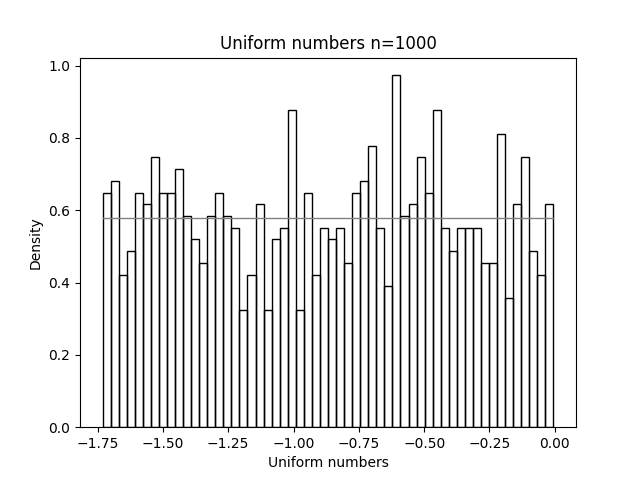
\includegraphics[scale=0.28]{Uniform1000}}
\caption{Равномерное распределение (\ref{eq:10}) для выборки мощности 1000}
\end{figure}

\newpage
\section{Обсуждение}
По результатам проведенной работы для всех распределений можно сделать вывод: чем больше выборка, тем ближе гистограмма к графику плотности вероятности. Гистограмма, построенная для маленькой выборки не показательна, т. к. по ней невозможно определить характер распределения. Также следует отметить, что максимумы гистограммы не совпали ни для одного распределения. А для распределения Коши и распределения Пуассона можно хорошо наблюдать всплески гистограммы.


\newpage
\begin{thebibliography}{4}
\addcontentsline{toc}{section}{\bibname}
\bibitem{cauchy}
Документация бибилиотеки scipy.stats.cauchy. 
\\ URL: https://docs.scipy.org/doc/scipy/reference/generated/scipy.stats.cauchy.html
\bibitem{laplace}
Документация бибилиотеки scipy.stats.laplace. 
\\ URL: https://docs.scipy.org/doc/scipy/reference/generated/scipy.stats.laplace.html
\bibitem{poisson}
Документация бибилиотеки scipy.stats.poisson.
\\ URL: https://docs.scipy.org/doc/scipy/reference/generated/scipy.stats.poisson.html
\bibitem{uniform}
Документация бибилиотеки scipy.stats.uniform.
\\ URL: https://docs.scipy.org/doc/scipy/reference/generated/scipy.stats.uniform.html
\end{thebibliography}
\end{document}
